\section{Mod\`ele \`a un plusieurs pools de MO}
\subsection{Description du mod\`ele}

\subsection{Simulation de r\'ef\'erence}

\begin{figure}[h!]
  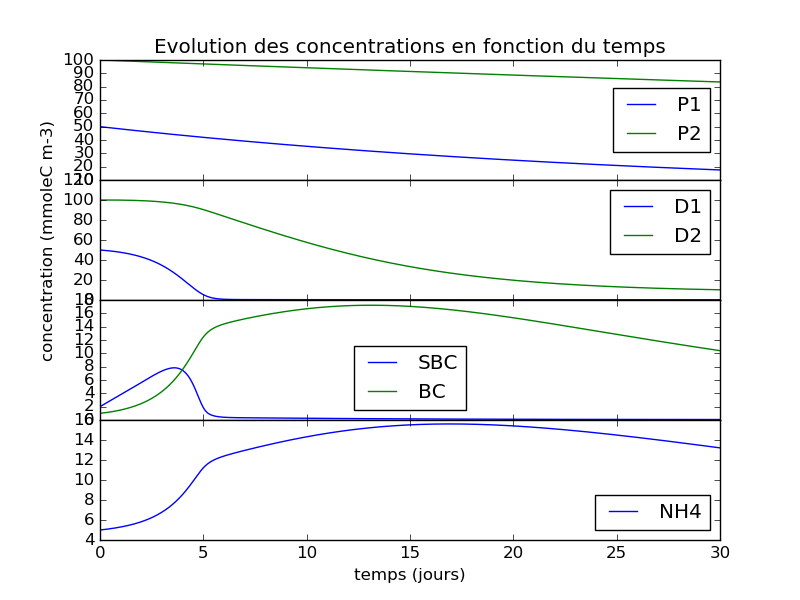
\includegraphics[width=\textwidth]{partie2/Ref.png}
  \caption{Simulation de r\'ef\'erence, pour un mod\`ele \`a plusieurs pools de mati\`ere organique
  }
  \label{fig:partie2ref}
\end{figure}

\par{
Les concentration en P1 et P2 diminuent selon une cin\'etique d'ordre 1. En effet, les \'equations de l'\'evolution de ces deux param\`etres sont toutes les deux d\'ependante d'une constante multipli\'ee par la concentration en P1 ou P2 (r\'ef aux \'equations). Cependant, nous pouvons constater que la concentration en P1 diminue plus rapidement que celle de P2 (la pente de la courbe est plus grande). Ceci s'explique par le fait que la constante dans l'\'equation de P1 est sup\'erieure \`a celle dans l'\'equation de P2. Donc, P1 est plus rapidement transform\'e en D1 que P2 est transform\'e en D2.
}
\par{
L'\'evolution des concentrations de D1 et D2 d\'ependent toutes les deux de deux termes, un correspondant \`a un apport depuis P1 ou P2, et un correspondant \`a leur hydrolyse en SBC. Les deux termes contribuent \`a l'\'evolution des concentrations en D1 et D2. Cependant, le terme d'hydrolyse en SBC est toujours plus important que le terme d'apport depuis P1 et P2, et c'est pourquoi, les concentrations en D1 et D2 d\'ecroissent tout le temps. De plus, nous pouvons constater que la concentration en D1 d\'ecroit plus rapidement que celle en D2. En effet, bien que la concentration initiale en D1 soit deux fois inf\'erieure \`a la concentration en D2, D1 est plus facilement biod\'egradable que D2 (emxD1 > emxD2 et khD1 < khD1). Ainsi, D1 est pr\'ef\'erentiellement hydrolys\'e en SBC pendant les premiers jours (jusque 3 jours environ), puis, lorsque la concentration en D1 devient tr\`es faible, les bact\'eries commencent \`a consommer D2. Lorsque D1 tombe \`a une concentration proche de 0 apr\`es 6 jours, D2 est plus rapidement hydrolys\'e en SBC qu'au d\'ebut de la simulation.
}
\par{
Pour ce qui est de l'\'evolution de la concentration en bact\'eries, celle-ci augmente rapidement jusque 5 jours, puis augmente plus lentement jusque 13 jours, atteignant alors un maximum de 17 mmolC.m-3, pour enfin diminuer relativement lentement. En effet, au d\'ebut de la simulation, la concentration en SBC cro\^it rapidement de 0 \`a 4 jours, atteignant un maximum de 8 mmolC.m-3, ce qui permet une croissance rapide des bact\'eries. Cette croissance rapide de la concentration en SBC est due \`a la concentration assez \'elev\'ee en D1 au d\'ebut de la simulation, bien que D2 contribue aussi au terme de croissance de la concentration en SBC. Lorsque la concentration en D1 se rapproche de 0, le terme d'\'evolution positive de la concentration en SBC n'est plus du qu'\`a D2, et c'est pourquoi la concentration en SBC diminue, jusqu'\`a se rapprocher de 0, ce qui entra\^ine un ralentissement de la croissance bact\'erienne. Finalement, apr\`es 13 jours, il n'y a plus assez de SBC pour permettre une croissance bact\'erienne sup\'erieure \`a la mortalit\'e, et c'est pourquoi la concentration en bact\'erie diminue.
}
\par{
Pour l'\'evolution de la concentration en NH4, celle-ci augmente rapidement au d\'ebut de la simulation, de 0 \`a 5 jours. La vitesse de croissance de NH4 va ensuite diminuer, pour atteindre un maximum de concentration de 14 mmolC.m-3 apr\`es 17 jours, pour enfin diminuer. Ainsi, ceci veut dire que le terme positif dans l'\'equation de l'\'evolution du NH4 est positif et sup\'erieur au terme de nitrification. Cela veut aussi dire que vNH4 est positif, et que donc les bact\'eries relarguent du NH4 dans leur environnement. Au d\'ebut de la simulation, la concentration en NH4 augmente rapidement car relativement beaucoup de bact\'eries sont pr\'esentes, et car la concentration en NH4 est faible, ce qui entra\^ine une valeur de nitrification faible. Ainsi, l'\'evolution de la concentration en NH4 va suivre l'\'evolution de la concentration en bact\'eries. Puis, la concentration va devenir relativement plus faible que celle en NH4, entrainant une diminution de la vitesse de croissance de la concentration en NH4. Finalement, la concentration en NH4 sera telle que l'\'evolution de cette concentration va devenir n\'egative.
}

\subsection{Tests de sensitivit\'e}
\subsubsection{Test 1}

\begin{figure}[h!]
  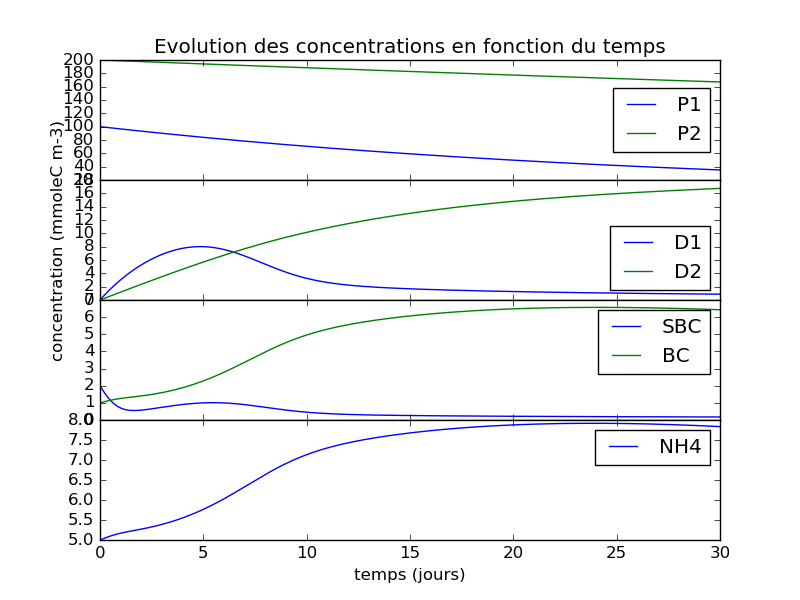
\includegraphics[width=\textwidth]{partie2/Test1.png}
  \caption{Simulation en doublant les concentrations initiales de P1 et P2, et en rendant celles de D1 et D2 nulles
  }
  \label{fig:partie2test1}
\end{figure}

\par{
Contrairement \`a la simulation de r\'ef\'erence, les concentrations initiales en P sont suffisantes pour permettre une augmentation de la concentration en D, de 0 \`a 5 jours pour D1 et tout le long de la simulation pour D2. En effet, apr\`es 5 jours, la concentration en P1 devient trop faible, coupl\'e \`a l'augmentation de la biomasse bact\'erienne, entra\^inant ainsi la diminution de la concentration en D1. Pour D2, le terme d'augmentation de la concentration est toujours sup\'erieur au terme de diminution.
}
\par{
En d\'ebut de simulation, nous pouvons observer une diminution de la concentration en SBC. En effet, celle-ci est principalement due \`a l'hydrolyse de D1. Or, la concentration initiale de D1 est nulle, ne permettant pas de croissance de SBC. Ainsi, la croissance des bact\'eries est lente. Apr\`es 1 jour, la concentration en SBC va augmenter, car l'hydrolyse de D1 et D2 est sup\'erieur \`a la consommation de SBC par les bact\'eries. Ceci va permettre aux bact\'eries de pr\'esenter une vitesse de croissance plus rapide. Ainsi, cette augmentation de la concentration en bact\'eries va devenir telle qu'elle va entra\^iner une diminution de la concentration en SBC. Cependant, contrairement \`a la simulation de r\'ef\'erence, la concentration de SBC rester suffisante pour permettre une croissance bact\'erienne jusque 25 jours.
}
\par{
De la m\^eme mani\`ere que pour la simulation de r\'ef\'erence, l'\'evolution de la concentration en NH4 va suivre une tendance semblable \`a l'\'evolution de la concentration en bact\'eries.
}

\subsubsection{Test 2}

\begin{figure}[h!]
  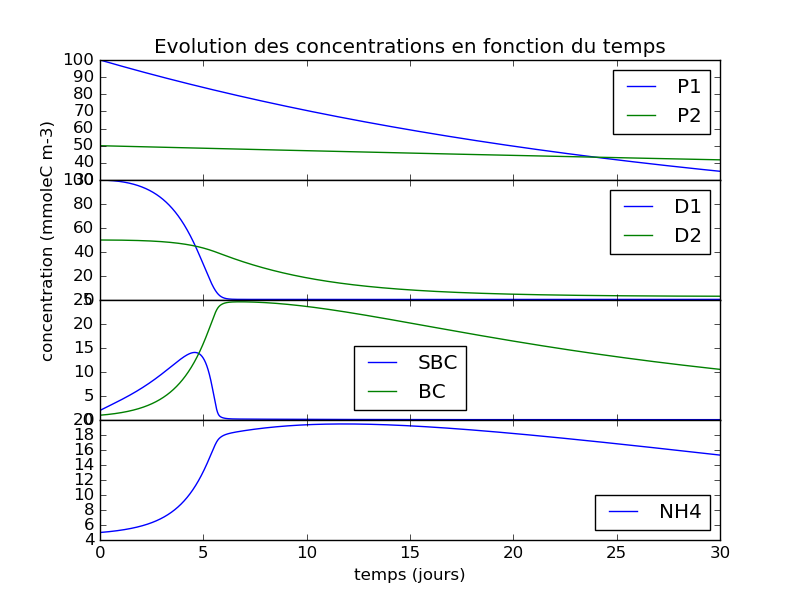
\includegraphics[width=\textwidth]{partie2/Test2.png}
  \caption{Simulation en doublant les concentrations initiales de P1 et D1, et en divisant par deux celles de P2 et D2
  }
  \label{fig:partie2test2}
\end{figure}

\par{
La concentration en P1 diminue relativement plus que P2, que dans le cas de la r\'ef\'erence. En effet, l'\'evolution de la concentration en P1 est directement proportionnelle \`a la concentration en P1, qui est ici initialement deux fois plus \'elev\'ee que dans le cas de la r\'ef\'erence. Comme la concentration en P1 est \'elev\'ee et que P1 est pr\'ef\'erentiellement hydrolys\'e en D1 puis en SBC que P2 en D2 puis en SBC, la concentration en P2 diminue tr\`es peu.
}
\par{
Bien que la concentration en P1 soit importante en d\'ebut de simulation, elle ne permet pas une croissance de D1. En effet, la concentration initiale en D1 est elle aussi plus importante que dans le cas de la simulation de r\'ef\'erence, ce qui augmente le terme n\'egatif dans l'\'equation de l'\'evolution de D1. Ainsi, D1 va d\'ecro\^itre rapidement pour atteindre une valeur proche de 0 apr\`es 6 jours. L'\'evolution de la concentration en D2 est quant \`a elle semblable \`a la simulation de r\'ef\'erence, bien que les concentrations initiales en P2 et D2 soient plus faibles.
}
\par{
La concentration en SBC va augmenter en d\'ebut de simulation, lorsque les concentrations en D1 et D2 sont importantes. Puis, puisque l'hydrolyse de D1 contribue de mani\`ere plus importante \`a l'augmentation de SBC, la concentration en SBC va diminuer lorsque celle en D1 atteint une valeur proche de 0. Ainsi, les bact\'eries vont cro\^itre lorsque la concentration en SBC augmente, et contrairement \`a la simulation de r\'ef\'erence, vont d\'ecroitre lorsque la concentration en SBC tombe proche de 0, car la concentration en D2 n'est plus suffisante pour maintenir une augmentation de la concentration en bact\'eries.
}

\subsubsection{Test 3}

\begin{figure}[h!]
  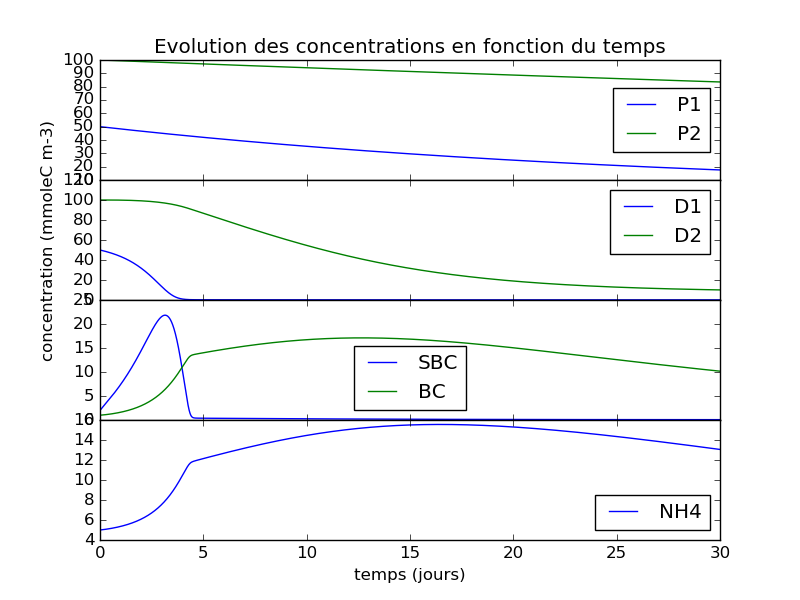
\includegraphics[width=\textwidth]{partie2/Test3.png}
  \caption{Simulation en doublant la valeur du param\`etre d'ectohydrolyse de D1 \`a temp\'erature optimale 
  }
  \label{fig:partie2test3}
\end{figure}

\par{
Nous avons augment\'e la biod\'egradabilit\'e de D1 par rapport \`a D2. Ainsi, la concentration en D1 va diminuer plus rapidement que dans le cas de la r\'ef\'erence, ce qui va entra\^iner un maximum de SBC plus grand, mais atteint plus rapidement. Puisque la concentration en SBC augmente plus rapidement que dans le cas de la simulation de r\'ef\'erence, la limite entre les deux types d'\'evolution positives des bact\'eries a lieu plus t\^ot aussi.
}

\subsubsection{Test 4}

\par{
\begin{figure}[h!]
  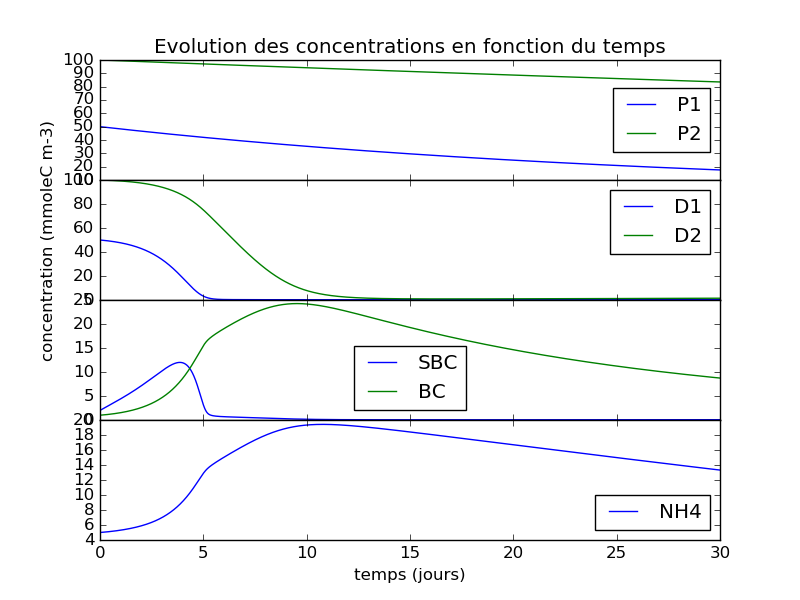
\includegraphics[width=\textwidth]{partie2/Test4.png}
  \caption{Simulation en r\'eduisant la valeur de la constante d'hydrolyse de D2
  }
  \label{fig:partie2test4}
\end{figure}
}
\par{
Contrairement au test pr\'ec\'edent, nous avons augment\'e la biod\'egradabilit\'e de D2 par rapport \`a D1. Ainsi, nous pouvons constater que l'\'evolution des concentrations de D1 et D2 sont plus semblables que dans le cas de la simulation de r\'ef\'erence. En effet, la concentration en D1 va diminuer plus rapidement, et va atteindre une concentration proche de 0 apr\`es 13 jours. Puisque D2 est mieux hydrolys\'e que lors de la r\'ef\'erence, il va contribuer de mani\`ere plus importante \`a l'augmentation de la concentration de SBC. Ainsi, bien que la concentration maximale en SBC soit atteinte en m\^eme temps que dans le cas de la r\'ef\'erence, car l'\'evolution de D1 est la m\^eme, la valeur de cette concentration maximale sera plus importante que dans le cas de la r\'ef\'erence. De la m\^eme mani\`ere, la concentration maximale en bact\'eries sera plus importante, mais atteinte plus rapidement que dans le cas de la simulation de r\'ef\'erence.
}

\subsubsection{Test 5}

\begin{figure}[h!]
  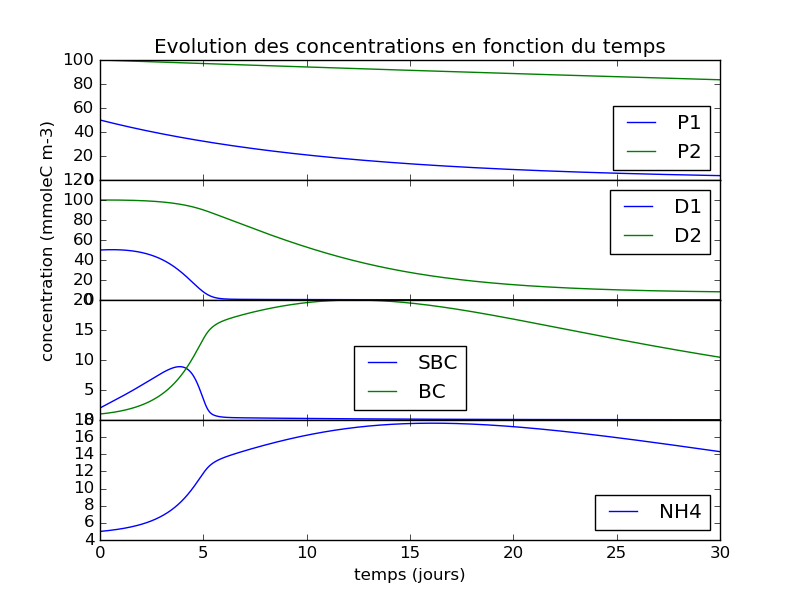
\includegraphics[width=\textwidth]{partie2/Test5.png}
  \caption{Simulation en augmentant la valeur de la constante d'endohydrolyse de P1 \`a temp\'erature optimale
  }
  \label{fig:partie2test5}
\end{figure}

\par{
Lors de cette simulation, nous avons augment\'e la vitesse d'hydrolyse de P1 en D1. Ainsi, nous pouvons constater que la concentration en P1 diminue plus rapidement que dans le cas de la r\'ef\'erence. En effet, dans la simulation de r\'ef\'erence, la diminution de la concentration en P1 \'etait presque lin\'eaire, tandis qu'elle ne l'est plus dans ce test.
}
\par{
Bien que les courbes de l'\'evolution de la concentration en D1 soient semblables entre ce test et la simulation de r\'ef\'erence, on peut constater que dans ce test, au tout d\'ebut de la simulation, la concentration en D1 diminue moins rapidement que dans le cas de la r\'ef\'erence. Ceci s'explique par le fait que l'hydrolyse de P1 en D1 est plus importante dans ce test, alors que l'hydrolyse de D1 en SBC se fait de la m\^eme mani\`ere que dans le cas de la r\'ef\'erence. Ainsi, le terme positif de l'\'evolution de la concentration de D1 est plus important que dans le cas de la simulation de r\'ef\'erence.
}
\par{
Puisque la concentration en D1 est plus importante en d\'ebut de simulation, la concentration en SBC l'est aussi. Ceci peut se remarquer sur le graphique de l'\'evolution de la concentration en SBC, sur lequel le maximum de concentration est sup\'erieur au cas de la r\'ef\'erence. Ainsi, la concentration maximale en bact\'eries est aussi sup\'erieure.
 
\subsection{Conclusion}
Qu'est ce qui contr\^ole la vitesse de croissance de BC (\'el\'ements les plus biod\'egradables) et qu'est ce qui contr\^ole le max de BC (lentement biod\'egradable)?

